\newcommand*{\PathToAssets}{../docs_src}%
\newcommand*{\PathToOutput}{../_output}%
% \newcommand*{\PathToBibFile}{../../../bibliography.bib}%


\documentclass[ignorenonframetext, 9pt]{beamer}
\usepackage{my_beamer_header}
\usepackage{my_common_header}


\title[FTSFR: Financial Forecasting Benchmark]{
Benchmarking Forecasting Methods for Financial Stability
}
\author[Bejarano et al.]{
  Jeremiah Bejarano\inst{1} \and
  Viren Desai\inst{2} \and
  Kausthub Keshava\inst{2} \and
  Arsh Kumar\inst{2} \and
  Zixiao Wang\inst{2} \and
  Vincent Hanyang Xu\inst{2} \and
  Yangge Xu\inst{2}
}
\institute[OFR]{
  \inst{1}Office of Financial Research, U.S. Department of the Treasury \and
  \inst{2}Independent
}
\date{\today}


\begin{document}
\begin{frame}[noframenumbering, plain]
\titlepage
\begin{tikzpicture}[remember picture,overlay]
  \node[anchor=south east,xshift=-0.5cm,yshift=0.5cm] at (current page.south east) {
    \includegraphics[height=1cm]{OFR_LOGO_WEB.png}
  };
\end{tikzpicture}
\end{frame}

\begin{frame}[noframenumbering, plain]
  \frametitle{Disclaimer}
  \centering
  \vspace{1cm}
  \large
  Any opinions expressed herein are my own and do not necessarily reflect those of the Office of Financial Research or the U.S. Department of the Treasury.
  \vspace{1cm}

  \normalsize
  All mistakes are my own.
\end{frame}

\begin{frame}
  \frametitle{Overview}
  \begin{itemize}
  \item \alert{Question:}
  Can modern global forecasting methods improve financial stability monitoring beyond traditional approaches?
  \item \alert{Approach:}
  Systematic benchmarking of 24 forecasting methods (classical to deep learning) on 27 canonical financial datasets with standardized evaluation.
  \item \alert{Main Result:}
  No universal best model; sophisticated methods achieve 3-10\% improvements over naive baselines, but gains are dataset-specific.
  \item \alert{Application:}
  Evidence-based guidance for financial stability authorities on which forecasting approaches work best for specific market segments.
  \end{itemize}
\end{frame}

% \begin{frame}[noframenumbering, plain]
%   \frametitle{Table of Contents}
%   \setbeamertemplate{section in toc}[sections numbered]
%   \tableofcontents%[hideallsubsections]
% \end{frame}

\section{Motivation}

\begin{frame}
\frametitle{Financial Stability Requires Forward-Looking Monitoring}
\begin{itemize}
\item Financial regulators increasingly emphasize \alert{forward-looking risk monitoring} to preemptively address systemic vulnerabilities
\vspace{0.3cm}
\item Early warning systems and predictive analytics are critical for timely policy responses
\vspace{0.3cm}
\item Effective forecasting enhances the toolkit for macroprudential surveillance and systemic risk monitoring
\vspace{0.3cm}
\item \alert{Better forecasting $\rightarrow$ Spot trouble earlier $\rightarrow$ Safeguard the economy}
\end{itemize}
\end{frame}

\begin{frame}
\frametitle{The Benchmarking Gap in Financial Forecasting}
\begin{itemize}
\item Time series forecasting is ubiquitous in finance, but lacks standardized evaluation frameworks
\vspace{0.2cm}
\item Current problem: Researchers evaluate methods on \alert{arbitrarily selected datasets}, making comparisons impossible
\vspace{0.2cm}
\item \alert{No Free Lunch Theorem}: Need domain-specific evaluation to identify what works in finance
\end{itemize}
\end{frame}

\begin{frame}
\frametitle{Existing Benchmarks Have Limited Financial Coverage}
\tiny
\begin{table}
\centering
\begin{tabular}{llp{4cm}}
\toprule
Source & Name & Coverage of Finance Domain \\
\midrule
McCracken (2016) & FRED-MD & US Macroeconomic Series \\
Hu et al. (2018) & FinTSB & Equities Returns only \\
Dau et al. (2019) & UCR Time Series Classification Archive & None \\
Bagnall et al. (2018) & UEA Multivariate Time Series Classification Archive & None \\
Godahewa et al. (2021) & Monash Time Series Forecasting Repository & Fred-MD is one component \\
Qiu et al. (2024) & TFB & NN5 Bank Cash Withdrawals, Equity (NYSE/NASDAQ), Foreign Exchange Rates \\
\bottomrule
\end{tabular}
\end{table}
\vspace{0.3cm}
\alert{Gap:} No comprehensive benchmark focused specifically on financial markets with canonical data cleaning procedures
\end{frame}

\begin{frame}
\frametitle{Why This Matters: Small Gains, Big Impact}
\begin{itemize}
\item Even 3-10\% forecasting improvements can be economically significant
\vspace{0.3cm}
\item In finance, small edges compound over time and across large portfolios
\vspace{0.3cm}
\item Standardized benchmarks drive progress by enabling:
\begin{itemize}
\item Apples-to-apples comparisons across methods
\item Identification of what works for specific market segments
\item Prevention of cherry-picking results
\end{itemize}
\vspace{0.3cm}
\item \alert{Solution}: Create comprehensive, literature-compliant financial forecasting benchmark
\end{itemize}
\end{frame}

\section{Related Literature}

\begin{frame}
  \frametitle{Three Key Research Streams}
  \begin{itemize}
  \item \alert{Financial Stability \& Many-Predictor Methods:}
  Principal components and factor models improve forecasts when exploiting many predictors.
  \\ \light{Stock \& Watson (2002); OFR's Financial Stress Index; Fed's SAFE system}
  \vspace{0.3cm}
  \item \alert{Return Predictability:}
  Modern asset pricing shows discount-rate variation drives return predictability across asset classes. Cross-sectional information enhances aggregate forecasts.
  \\ \light{Cochrane (2011); Kelly \& Pruitt (2013); Kelly \& Xiu (2023)}
  \vspace{0.3cm}
  \item \alert{Global Time Series Forecasting:}
  Single models trained across many series consistently win forecasting competitions. Particularly effective for related financial series sharing economic drivers.
  \\ \light{M-competitions; NN3/NN5 competitions; Godahewa et al. (2021)}
  \end{itemize}
\end{frame}

\section{Data \& Contributions}


\begin{frame}
  \frametitle{Comprehensive Financial Dataset Coverage}
  \begin{itemize}
  \item \alert{27 datasets} across multiple asset classes and market segments:
  \vspace{0.1cm}
  \begin{itemize}
    \item \textbf{Asset Returns:} Equities (CRSP), Corporate \& Treasury bonds, CDS, Options, FX, Commodities
    \item \textbf{Arbitrage Spreads:} CIP deviations, CDS-bond basis, Treasury-swap spreads, TIPS-Treasury
    \item \textbf{Financial Stability Data:} Bank call reports, intermediary risk factors, yield curves
  \end{itemize}
  \vspace{0.2cm}
  \item Each dataset follows \alert{canonical cleaning procedures} from seminal finance papers
  \vspace{0.1cm}
  \item Validated by replicating key results from original studies
  \vspace{0.1cm}
  \item Scale: From 4 commodity series to 6,388 individual CDS contracts
  \end{itemize}
\label{slide:data_overview}
\end{frame}

\begin{frame}
  \frametitle{Dataset Overview}
  \begin{itemize}
  \item \alert{27 datasets} across multiple asset classes
  \item Each follows canonical cleaning procedures from seminal papers
  \item Three main categories:
  \begin{itemize}
    \item Returns data (11 datasets)
    \item Basis spread data (5 datasets)
    \item Other financial data (11 datasets)
  \end{itemize}
  \item Next slides show detailed dataset listings
  \end{itemize}
\end{frame}

\begin{frame}[plain]
  \tiny
  \begin{table}
  \centering
  \begin{tabular}{p{2.5cm}p{5cm}p{2.5cm}}
  \toprule
  Dataset Name & Description & Citation \\
  \midrule
  \multicolumn{3}{c}{\textbf{Returns Data}} \\
  \midrule
  CDS Contract & Monthly returns for individual CDS contracts & Palhares (2012) \\
  CDS Portfolio & Aggregated into 20 CDS portfolios by tenor and credit quality & He et al. (2017) \\
  Commodity & Monthly returns for commodity futures & Yang (2013) \\
  Corporate Bond & Monthly returns for individual corporate bonds from TRACE & Dickerson et al. (2024) \\
  Corporate Portfolio & Corporate bond portfolios by credit spread & Nozawa (2017) \\
  CRSP Stock & Monthly stock returns from CRSP database & Fama \& French (1993) \\
  FF25 Size-BM & Daily Fama-French 25 portfolios: size and book-to-market & ibid. \\
  FX & Daily foreign exchange returns vs USD & Lettau et al. (2014) \\
  SPX Options & Monthly returns for individual SPX option contracts & Constantinides et al. (2013) \\
  Treasury Bond & Monthly returns for individual Treasury bonds from CRSP & Gürkaynak et al. (2007) \\
  Treasury Portfolio & Monthly returns for Treasury bond portfolios by maturity & ibid. \\
  \bottomrule
  \end{tabular}
  \end{table}
\end{frame}

\begin{frame}[plain]
  \tiny
  \begin{table}
  \centering
  \begin{tabular}{p{2.5cm}p{5cm}p{2.5cm}}
  \toprule
  Dataset Name & Description & Citation \\
  \midrule
  \multicolumn{3}{c}{\textbf{Basis Spread Data}} \\
  \midrule
  CDS-Bond & Monthly CDS-bond basis spreads & Siriwardane et al. (2021) \\
  CIP & Monthly covered interest parity deviations & Du et al. (2018) \\
  TIPS-Treasury & Monthly TIPS-Treasury basis spreads & Fleckenstein et al. (2014) \\
  Treasury-SF & Monthly Treasury-SF arbitrage spreads & Fleckenstein et al. (2020) \\
  Treasury-Swap & Monthly Treasury-Swap arbitrage spreads & Siriwardane et al. (2021) \\
  \midrule
  \multicolumn{3}{c}{\textbf{Other Financial Data}} \\
  \midrule
  Bank Cash Liquidity & Quarterly cash liquidity from call report data & Drechsler et al. (2017) \\
  Bank Leverage & Quarterly leverage ratios from call report data & ibid. \\
  BHC Cash Liquidity & Quarterly bank holding company cash liquidity & ibid. \\
  BHC Leverage & Quarterly bank holding company leverage ratios & ibid. \\
  HKM Daily Factor & Intermediary risk factors, including capital ratio, capital risk factor & He et al. (2017) \\
  Treasury Yield Curve & Daily Nelson-Siegel-Svensson zero-coupon yields, 1-30 years & Gürkaynak et al. (2007) \\
  \bottomrule
  \end{tabular}
  \end{table}
\end{frame}

\begin{frame}
  \frametitle{Dataset Statistics}
  \begin{itemize}
  \item Scale varies dramatically across datasets
  \item From 4 commodity series to 6,388 individual CDS contracts
  \item Both portfolio-level and security-level data
  \item Train/test splits provide substantial out-of-sample periods
  \item Next slide shows detailed statistics
  \end{itemize}
\end{frame}

\begin{frame}[plain]
  \centering
  \vspace{0.2cm}
  \scalebox{0.9}{%
    % Dataset Statistics Summary - tabular content only
% Generated automatically by create_dataset_statistics.py
\footnotesize
\setlength{\tabcolsep}{1.2pt}
\renewcommand{\arraystretch}{0.9}
\begin{tabular}{@{}llrrrrll@{}}
\toprule
 & Frequency & \begin{tabular}[c]{@{}r@{}}Unique\\Entities\end{tabular} & \begin{tabular}[c]{@{}r@{}}Min\\Length\end{tabular} & \begin{tabular}[c]{@{}r@{}}Median\\Length\end{tabular} & \begin{tabular}[c]{@{}r@{}}Max\\Length\end{tabular} & Min Date & Max Date \\
\midrule
\multicolumn{8}{l}{\textbf{Basis Spreads}} \\
CDS-Bond & Monthly & 3402 & 1 & 16 & 169 & 2002-09-30 & 2022-09-30 \\
CIP & Monthly & 8 & 3997 & 5732 & 6030 & 2001-12-04 & 2025-02-28 \\
TIPS-Treasury & Monthly & 4 & 5126 & 5162 & 5197 & 2004-07-21 & 2025-05-30 \\
Treasury-SF & Monthly & 5 & 3783 & 5185 & 5192 & 2004-06-23 & 2025-01-08 \\
Treasury-Swap & Monthly & 7 & 1353 & 4482 & 6164 & 2001-12-20 & 2025-08-11 \\
\midrule
\multicolumn{8}{l}{\textbf{Returns (Portfolios)}} \\
CDS Portfolio & Monthly & 20 & 275 & 275 & 276 & 2001-01-01 & 2023-12-01 \\
Corporate Portfolio & Monthly & 10 & 242 & 242 & 242 & 2002-08-31 & 2022-09-30 \\
FF25 Size-BM & Daily & 25 & 26023 & 26023 & 26023 & 1926-07-01 & 2025-06-30 \\
SPX Options Portfolios & Monthly & 18 & 288 & 288 & 288 & 1996-01-31 & 2019-12-31 \\
Treasury Portfolio & Monthly & 10 & 657 & 664 & 666 & 1970-01-31 & 2025-06-30 \\
\midrule
\multicolumn{8}{l}{\textbf{Returns (Disaggregated)}} \\
CDS Contract & Monthly & 6552 & 1 & 25 & 96 & 2001-01-01 & 2023-12-01 \\
CRSP Stock & Monthly & 26757 & 1 & 85 & 1188 & 1926-01-30 & 2024-12-31 \\
CRSP Stock (ex-div) & Monthly & 26757 & 1 & 85 & 1188 & 1926-01-30 & 2024-12-31 \\
Commodity & Monthly & 23 & 283 & 511 & 668 & 1970-01-30 & 2025-08-12 \\
Corporate Bond & Monthly & 23473 & 1 & 36 & 242 & 2002-08-31 & 2022-09-30 \\
FX & Monthly & 9 & 4029 & 5991 & 6789 & 1999-02-09 & 2025-02-28 \\
Treasury Bond & Monthly & 2044 & 1 & 37 & 364 & 1970-01-31 & 2025-06-30 \\
\midrule
\multicolumn{8}{l}{\textbf{Other}} \\
BHC Cash Liquidity & Quarterly & 13770 & 1 & 46 & 177 & 1976-03-31 & 2020-03-31 \\
BHC Leverage & Quarterly & 13761 & 1 & 46 & 177 & 1976-03-31 & 2020-03-31 \\
Bank Cash Liquidity & Quarterly & 23862 & 1 & 66 & 177 & 1976-03-31 & 2020-03-31 \\
Bank Leverage & Quarterly & 22965 & 1 & 67 & 177 & 1976-03-31 & 2020-03-31 \\
HKM All Factor & Monthly & 4 & 516 & 516 & 516 & 1970-01-01 & 2012-12-01 \\
HKM Daily Factor & Daily & 4 & 4765 & 4766 & 4766 & 2000-01-03 & 2018-12-11 \\
HKM Monthly Factor & Monthly & 4 & 587 & 587 & 587 & 1970-01-01 & 2018-11-01 \\
Treasury Yield Curve & Daily & 30 & 9912 & 12206 & 16002 & 1961-06-14 & 2025-08-08 \\
\bottomrule
\end{tabular}%
  }
\end{frame}

\begin{frame}
  \frametitle{Key Innovation: Literature-Compliant Data Curation}
  \begin{itemize}
  \item \alert{Not doing anything novel is a FEATURE, not a bug}
  \vspace{0.2cm}
  \item Each dataset uses exact methodology from canonical finance papers:
  \begin{itemize}
    \item Equities: Fama \& French (1993) filters
    \item Treasuries: Gürkaynak et al. (2007) procedure
    \item Corporate bonds: Market microstructure noise correction
    \item CDS: Palhares (2012) constant-risky-duration construction
  \end{itemize}
  \vspace{0.2cm}
  \item Enables \alert{exact replication} of established results
  \vspace{0.1cm}
  \item Addresses finance's potential replication crisis through standardized, open-source data infrastructure
  \end{itemize}
\end{frame}

\begin{frame}
  \frametitle{Data Quality: SPX Options Market Growth}
  \centering
  
\includegraphics[width=0.8\textwidth]{\PathToAssets/spx_options_over_time.png}

  \vspace{0.3cm}
  Massive growth: 72 option portfolios from 19 million individual contracts (1996-2019)
\end{frame}

\begin{frame}
  \frametitle{Data Quality: Treasury Basis Validation}
  \centering
  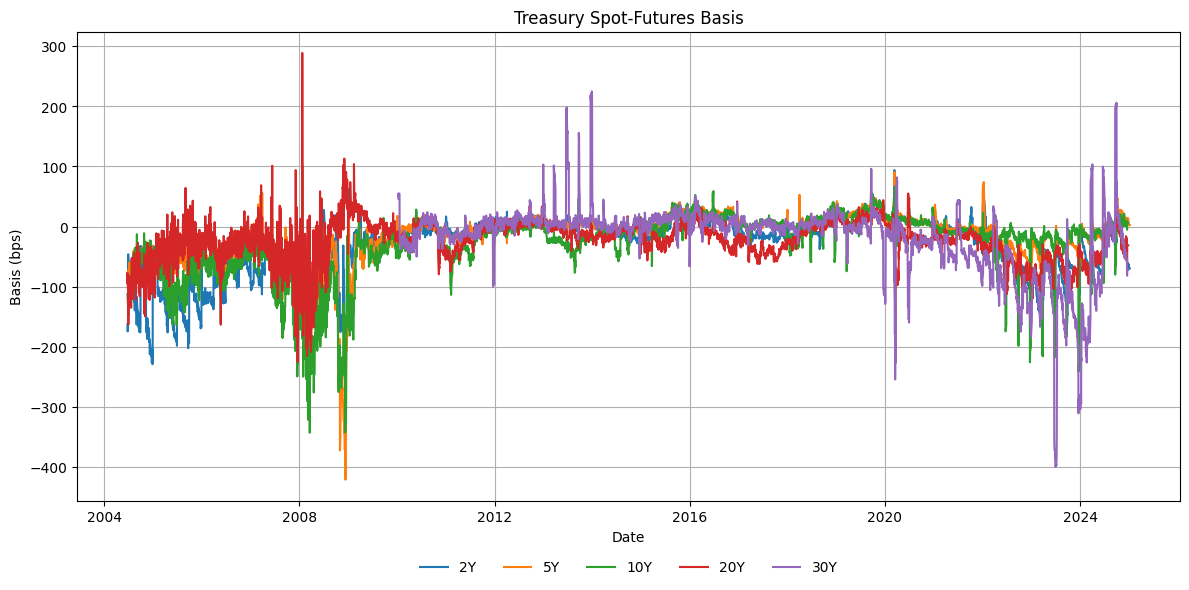
\includegraphics[width=0.8\textwidth]{\PathToAssets/treasury_spot_futures_arbitrage.png}

  \vspace{0.3cm}
  Successfully replicates Treasury spot-futures basis patterns from literature
\end{frame}

\begin{frame}
  \frametitle{Open Source Implementation}
  \begin{itemize}
  \item \alert{Fully reproducible} data pipeline: automated download, cleaning, formatting
  \vspace{0.2cm}
  \item Available on GitHub: \texttt{github.com/jmbejara/ftsfr}
  \vspace{0.2cm}
  \item Handles data licensing constraints:
  \begin{itemize}
    \item Provides scripts rather than redistributing proprietary data
    \item Works with institutional subscriptions (WRDS, Bloomberg)
    \item Enables exact dataset reproduction across researchers
  \end{itemize}
  \vspace{0.2cm}
  \item Both \alert{aggregated portfolios} (for replication) and \alert{disaggregated data} (for global forecasting)
  \vspace{0.1cm}
  \item Virtual environments ensure perfect reproducibility
  \end{itemize}
\end{frame}

\section{Methodology}


\begin{frame}{Forecasting Methods: 24 Models Across Three Categories}
\begin{itemize}
\item \alert{Classical Statistical Methods:}
\begin{itemize}
  \item Naive, Seasonal Naive, Theta, Simple Exponential Smoothing, Auto-ARIMA
  \item Computationally efficient, interpretable, strong baselines
\end{itemize}
\vspace{0.3cm}
\item \alert{Machine Learning:}
\begin{itemize}
  \item Linear models, gradient boosting (e.g., CatBoost)
  \item Balance between complexity and interpretability
\end{itemize}
\vspace{0.3cm}
\item \alert{Deep Learning (Global Methods):}
\begin{itemize}
  \item Transformer, N-BEATS, N-HiTS, TiDE, KAN, DLinear, NLinear
  \item Train single model across all time series in dataset
  \item Learn cross-sectional patterns and spillover effects
\end{itemize}
\end{itemize}
\end{frame}

\begin{frame}
  \frametitle{Evaluation Framework}
  \begin{itemize}
  \item \alert{Consistent data preprocessing:} All models receive identical filtered datasets
  \vspace{0.3cm}
  \item \alert{Fair comparison methodology:}
  \begin{itemize}
    \item Adaptive filtering based on median entity length
    \item Seasonality-aware forecast horizons
    \item Protection for small datasets ($\leq$10 entities)
  \end{itemize}
  \vspace{0.3cm}
  \item \alert{Two complementary error metrics:}
  \begin{itemize}
    \item MASE: Standard in time series forecasting (robust to outliers)
    \item Out-of-sample $R^2$: Standard in finance (emphasizes large errors)
  \end{itemize}
  \vspace{0.3cm}
  \item \alert{Focus on baseline performance} with minimal hyperparameter tuning
  \end{itemize}
\end{frame}

\begin{frame}
  \frametitle{Data Preprocessing for Fair Comparison}
  \begin{itemize}
  \item Consistent filtering across all models ensures fairness
  \item Removes series too short for reliable forecasting
  \item Protects small datasets ($\leq$10 entities) from elimination
  \item Impact varies by dataset:
  \begin{itemize}
    \item Portfolio-level: minimal filtering needed
    \item Disaggregated: more filtering due to short-lived securities
  \end{itemize}
  \item Next slide shows filtering impact statistics
  \end{itemize}
\end{frame}

\begin{frame}[plain]
    \centering
    \vspace{0.2cm}
    \scalebox{0.9}{%
    % Filtered Dataset Statistics Summary - tabular content only
% Generated automatically by create_filtered_dataset_statistics.py
\footnotesize
\setlength{\tabcolsep}{1.0pt}
\renewcommand{\arraystretch}{0.9}
\begin{tabular}{@{}llrrrrlll@{}}
\toprule
 & Frequency & \begin{tabular}[c]{@{}r@{}}Entities\\Before\end{tabular} & \begin{tabular}[c]{@{}r@{}}Entities\\After\end{tabular} & \begin{tabular}[c]{@{}r@{}}Median Length\\Before\end{tabular} & \begin{tabular}[c]{@{}r@{}}Median Length\\After\end{tabular} & Min Date & Max Date \\
\midrule
\multicolumn{8}{l}{\textbf{Basis Spreads}} \\
CDS-Bond & Monthly & 3398 & 3314 & 199 & 201 & 2002-09-30 & 2022-09-30 \\
CIP & Monthly & 8 & 8 & 224 & 224 & 2001-12-04 & 2025-02-22 \\
TIPS-Treasury & Monthly & 4 & 4 & 200 & 200 & 2004-07-21 & 2025-05-21 \\
Treasury-SF & Monthly & 5 & 5 & 204 & 204 & 2004-06-23 & 2024-12-23 \\
Treasury-Swap & Monthly & 7 & 7 & 166 & 166 & 2001-12-20 & 2025-08-04 \\
\midrule
\multicolumn{8}{l}{\textbf{Returns (Portfolios)}} \\
CDS Portfolio & Monthly & 20 & 20 & 220 & 220 & 2001-01-01 & 2023-12-01 \\
Corporate Portfolio & Monthly & 10 & 10 & 193 & 193 & 2002-08-31 & 2022-09-30 \\
FF25 Size-BM & Daily & 25 & 25 & 28928 & 28928 & 1926-07-01 & 2025-06-30 \\
SPX Options Portfolios & Monthly & 18 & 18 & 230 & 230 & 1996-01-31 & 2019-12-31 \\
Treasury Portfolio & Monthly & 10 & 10 & 532 & 532 & 1970-01-31 & 2025-06-30 \\
\midrule
\multicolumn{8}{l}{\textbf{Returns (Disaggregated)}} \\
CDS Contract & Monthly & 6508 & 6388 & 215 & 217 & 2001-01-01 & 2023-12-01 \\
CRSP Stock & Monthly & 26719 & 26474 & 436 & 440 & 1926-01-30 & 2024-12-31 \\
CRSP Stock (ex-div) & Monthly & 26719 & 26474 & 436 & 440 & 1926-01-30 & 2024-12-31 \\
Commodity & Monthly & 23 & 4 & 399 & 555 & 1970-01-30 & 2025-07-30 \\
Corporate Bond & Monthly & 23445 & 22146 & 144 & 154 & 2002-08-31 & 2022-09-30 \\
FX & Monthly & 9 & 9 & 222 & 222 & 1999-02-09 & 2025-02-23 \\
Treasury Bond & Monthly & 2033 & 1951 & 234 & 250 & 1970-01-31 & 2025-06-30 \\
\midrule
\multicolumn{8}{l}{\textbf{Other}} \\
BHC Cash Liquidity & Quarterly & 13529 & 13279 & 136 & 136 & 1976-03-31 & 2020-03-31 \\
BHC Leverage & Quarterly & 13520 & 13270 & 136 & 136 & 1976-03-31 & 2020-03-31 \\
Bank Cash Liquidity & Quarterly & 23834 & 23816 & 168 & 168 & 1976-03-31 & 2020-03-31 \\
Bank Leverage & Quarterly & 22940 & 22927 & 168 & 168 & 1976-03-31 & 2020-03-31 \\
HKM All Factor & Monthly & 4 & 4 & 412 & 412 & 1970-01-01 & 2012-12-01 \\
HKM Daily Factor & Daily & 4 & 4 & 5534 & 5534 & 2000-01-03 & 2018-12-11 \\
HKM Monthly Factor & Monthly & 4 & 4 & 469 & 469 & 1970-01-01 & 2018-11-01 \\
Treasury Yield Curve & Daily & 30 & 30 & 13180 & 13180 & 1961-06-14 & 2025-08-08 \\
\bottomrule
\end{tabular}
    }
  \end{frame}

\begin{frame}
  \frametitle{Error Metrics: Mathematical Definitions}
  \begin{itemize}
  \item \alert{Mean Absolute Scaled Error (MASE):}
  \[
  \mathrm{MASE}=\frac{\frac{1}{T}\sum_{t=1}^T |y_t-\hat y_t|}
  {\displaystyle \frac{1}{N-s}\sum_{t=s+1}^{N} |y_t - y_{t-s}|}
  \]
  \begin{itemize}
    \item \textbf{Why chosen:} Standard accuracy measure in time series forecasting \textcolor{gray}{(Hyndman \& Koehler 2006)}
    \item Scale-free comparison across different financial series
    \item Robust to outliers (uses absolute errors)
    \item Values $<1$ indicate improvement over naive benchmark
  \end{itemize}
  \vspace{0.3cm}
  \item \alert{Out-of-Sample $R^2$:}
  \[
  R^2_{\text{oos}} = 1 - \frac{\sum_{t=1}^T (y_t-\hat y_t)^2}{\sum_{t=1}^T (y_t-\bar{y}_{\text{train}})^2}
  \]
  \begin{itemize}
    \item \textbf{Why chosen:} Standard for evaluating predictive models in finance \textcolor{gray}{(Campbell \& Thompson 2008)}
    \item Measures percentage reduction in MSE vs historical average
    \item Emphasizes large forecast errors (quadratic loss)
    \item Positive values indicate outperformance of simple benchmark
  \end{itemize}
  \end{itemize}
\end{frame}

\section{Results}


\begin{frame}
  \frametitle{Key Finding: No Universal Best Model}
  \centering
  \includegraphics[width=0.9\textwidth]{\PathToOutput/forecasting2/relative_mase_heatmap.png}
  \vspace{0.2cm}

  Performance relative to Naive baseline (blue = better, red = worse)
\end{frame}

\begin{frame}
  \frametitle{Main Results}
  \begin{itemize}
  \item \alert{No Free Lunch confirmed:} Model performance varies significantly by dataset characteristics
  \vspace{0.3cm}
  \item \alert{Naive baseline is remarkably competitive}, especially for returns data where market efficiency limits predictability
  \vspace{0.3cm}
  \item \alert{When sophisticated models win:}
  \begin{itemize}
    \item Disaggregated datasets (thousands of entities) benefit from global methods
    \item 10-15\% improvements over naive for CRSP Stock, Corporate Bond data
    \item Cross-sectional learning adds value
  \end{itemize}
  \vspace{0.3cm}
  \item \alert{Asset class differences:}
  \begin{itemize}
    \item Basis spreads \& yield curves: Higher predictability
    \item Equity \& options returns: More challenging
    \item Portfolio-level data: Limited gains from complexity
  \end{itemize}
  \end{itemize}
\end{frame}

\begin{frame}
  \frametitle{Economic Significance of Small Improvements}
  \begin{itemize}
  \item Typical improvements: \alert{3-10\% better than naive baselines}
  \vspace{0.3cm}
  \item Why this matters in finance:
  \begin{itemize}
    \item Small edges compound over time
    \item Large portfolios amplify benefits
    \item Institutional scale makes modest gains valuable
  \end{itemize}
  \vspace{0.3cm}
  \item \alert{Model insights by type:}
  \begin{itemize}
    \item Traditional methods (Theta, ARIMA): Still competitive
    \item Deep learning: Mixed results, dataset-dependent
    \item Linear deep models (DLinear/NLinear): Surprisingly effective
    \item Complex architectures may not align with financial time series characteristics
  \end{itemize}
  \end{itemize}
\end{frame}

\begin{frame}
  \frametitle{Detailed Performance Results}
  \begin{itemize}
  \item MASE: Performance compared to Naive baseline
  \begin{itemize}
    \item Values $<$ 1.0 = better than Naive
    \item Values $>$ 1.0 = worse than Naive
  \end{itemize}
  \item Out-of-sample $R^2$: Percentage reduction in MSE vs historical average
  \begin{itemize}
    \item Positive values = model outperforms benchmark
    \item Negative values = model underperforms benchmark
  \end{itemize}
  \item Following slides show detailed tables for both metrics
  \end{itemize}
\end{frame}

\begin{frame}[plain]
  \tiny
  \vspace{-0.5cm}
  \centering
  \textbf{Relative MASE Results by Dataset and Model}\\
  \vspace{0.2cm}
  % Relative MASE Results by Dataset and Model - tabular content only
% Generated automatically by create_results_tables2.py
\scriptsize
\setlength{\tabcolsep}{1.5pt}
\renewcommand{\arraystretch}{0.9}
\begin{tabular}{@{}lrrrrrrrrrrr@{}}
\toprule
 & Theta & SES & ARIMA & DeepAR & NBEATS & NHITS & DLinear & NLinear & Transformer & TiDE & KAN \\
\midrule
\multicolumn{12}{l}{\textbf{Basis Spreads}} \\
CDS-Bond & 1.14 & 1.07 & 1.27 & 2.43 & \textbf{1.00} & 1.02 & 2.43 & 1.03 & 1.55 & 1.93 & 1.33 \\
CIP & 0.96 & 0.97 & \textbf{0.88} & 1.83 & 1.83 & 1.45 & 1.37 & 1.32 & 1.49 & 1.42 & 3.65 \\
TIPS-Treasury & 1.04 & 1.00 & 1.29 & 5.36 & 1.17 & \textbf{0.91} & 1.50 & 2.96 & 1.40 & 1.23 & 1.61 \\
\midrule
\multicolumn{12}{l}{\textbf{Returns (Portfolios)}} \\
CDS Portfolio & 0.68 & 0.64 & 0.64 & \textbf{0.61} & 0.62 & 0.61 & 0.62 & 0.76 & 0.66 & 0.62 & 0.63 \\
Corporate Portfolio & 0.97 & 0.97 & 0.98 & 1.00 & 1.01 & 1.00 & 0.97 & 0.98 & 1.00 & \textbf{0.96} & 1.01 \\
FF25 Size-BM & 0.85 & 0.85 & \textbf{0.85} & 0.88 & 0.85 & 0.85 & 0.85 & 0.85 & -- & 0.85 & 0.85 \\
SPX Options Portfolios & 1.12 & 1.00 & 1.00 & 1.06 & \textbf{0.99} & 1.00 & 1.02 & 1.00 & 1.00 & 1.02 & 1.01 \\
Treasury Portfolio & 1.06 & 0.99 & 1.01 & 1.03 & 0.98 & \textbf{0.97} & 0.99 & 0.99 & 1.02 & 0.99 & 1.00 \\
\midrule
\multicolumn{12}{l}{\textbf{Returns (Disaggregated)}} \\
CDS Contract & 0.93 & 0.97 & 1.21 & 2.84 & 0.96 & 0.93 & 1.04 & 1.02 & \textbf{0.88} & 1.07 & 0.89 \\
CRSP Stock & 0.99 & 0.98 & 0.94 & 0.89 & 1.01 & 1.03 & 0.99 & \textbf{0.86} & 0.88 & 0.93 & 0.90 \\
CRSP Stock (ex-div) & 0.99 & 0.98 & 0.94 & 0.88 & 1.03 & 1.05 & 0.99 & \textbf{0.85} & 0.88 & 0.91 & 0.91 \\
Commodity & 1.01 & 1.00 & \textbf{0.83} & 6.99 & 0.92 & 1.08 & 1.20 & 1.13 & 1.17 & 1.41 & 1.10 \\
Corporate Bond & \textbf{0.55} & 0.60 & 0.73 & 0.60 & 0.92 & 0.89 & 0.81 & 0.91 & 0.76 & 0.65 & 0.81 \\
FX & 1.11 & 1.00 & 1.09 & \textbf{0.97} & 1.10 & 1.18 & 1.05 & 1.06 & 1.06 & 1.02 & 1.15 \\
Treasury Bond & 0.86 & 0.88 & 1.11 & 1.03 & 0.83 & 0.74 & 1.21 & 1.63 & 0.79 & \textbf{0.39} & 1.12 \\
\midrule
\multicolumn{12}{l}{\textbf{Other}} \\
BHC Cash Liquidity & 0.96 & \textbf{0.95} & 0.98 & 1.18 & 0.96 & 0.97 & 1.21 & 1.04 & 0.98 & 1.12 & 0.97 \\
BHC Leverage & 1.06 & 1.00 & 1.05 & 2.16 & 0.96 & 0.97 & 1.40 & 1.11 & \textbf{0.92} & 1.07 & 1.00 \\
Bank Cash Liquidity & 0.96 & \textbf{0.95} & 1.00 & 1.17 & 0.97 & 0.97 & 1.15 & 1.04 & 0.97 & 1.08 & 0.99 \\
Bank Leverage & 0.96 & 0.98 & 1.04 & 4.14 & 0.95 & \textbf{0.94} & 1.54 & 1.11 & 0.97 & 1.29 & 0.99 \\
HKM All Factor & 1.08 & 0.99 & 1.00 & 0.97 & 1.19 & \textbf{0.64} & 0.93 & 0.98 & 0.96 & 0.93 & 1.15 \\
HKM Daily Factor & 1.51 & 1.00 & 1.00 & 1.04 & \textbf{0.99} & 1.04 & 1.02 & 1.00 & 1.22 & 1.01 & 1.05 \\
HKM Monthly Factor & 0.93 & 0.96 & 0.95 & 0.55 & 1.27 & 1.91 & 0.27 & 0.63 & 1.29 & \textbf{0.24} & 0.93 \\
Treasury Yield Curve & 1.27 & \textbf{1.00} & 1.90 & 1.02 & 1.81 & 2.05 & 1.03 & 1.01 & -- & -- & 2.02 \\
\bottomrule
\end{tabular}
\end{frame}

% \begin{frame}[plain]

%     \centering
%     \textbf{Out-of-Sample $R^2$ Results by Dataset and Model}\\
%     \vspace{0.2cm}
%     \scalebox{0.9}{%
%       \input{../_output/forecasting2/r2_oos_pivot_tabular.tex}%
%     }
%   \end{frame}


\begin{frame}
  \frametitle{Practical Guidance for Financial Stability Monitoring}
  \begin{itemize}
  \item \alert{For disaggregated financial data:} Global methods can provide meaningful improvements
  \vspace{0.3cm}
  \item \alert{For portfolio-level indicators:} Simple methods often sufficient
  \vspace{0.3cm}
  \item \alert{For basis spreads \& yield curves:} Higher predictability makes sophisticated methods worthwhile
  \vspace{0.3cm}
  \item \alert{For equity returns:} Naive baselines hard to beat (market efficiency)
  \vspace{0.3cm}
  \item \alert{Key takeaway:} Match method complexity to data characteristics and economic context
  \end{itemize}
\end{frame}

\section{Conclusions}

\begin{frame}
  \frametitle{Contributions \& Future Work}
  \begin{itemize}
  \item \alert{Main Contributions:}
  \begin{itemize}
    \item First comprehensive financial time series forecasting benchmark
    \item 27 datasets with canonical academic cleaning procedures
    \item Evidence that model choice depends critically on data characteristics
    \item Open-source implementation enabling reproducible research
  \end{itemize}
  \vspace{0.3cm}
  \item \alert{For practitioners:} Evidence-based guidance on forecasting method selection for financial stability monitoring
  \vspace{0.3cm}
  \item \alert{Future work:}
  \begin{itemize}
    \item Expand coverage to international markets
    \item Multi-step and long-horizon forecasting
    \item Integration with stress testing frameworks
    \item Real-time updating and monitoring systems
  \end{itemize}
  \end{itemize}
\end{frame}

\appendix
\begin{frame}
  \centering
  \textbf{Appendix}
\end{frame}

\begin{frame}
  \frametitle{Dataset Statistics Summary}
  \label{slide:dataset_stats}
\small
\begin{itemize}
\item \alert{Scale varies dramatically across datasets:}
\begin{itemize}
  \item Commodities: 4 series (GSCI-based)
  \item CDS Contracts: 6,388 individual contracts
  \item CRSP Stock: 4,000+ individual equities
  \item Corporate Bonds: 1,000+ individual bonds
\end{itemize}
\vspace{0.3cm}
\item \alert{Time coverage:} Most datasets span 10-25 years
\vspace{0.3cm}
\item \alert{Frequency:} Daily (FX, yield curves) to quarterly (bank data)
\vspace{0.3cm}
\item \alert{Two levels of aggregation:}
\begin{itemize}
  \item Portfolio-level (10-50 series) for replication
  \item Security-level (100s-1000s) for global forecasting
\end{itemize}
\end{itemize}
\end{frame}

\begin{frame}
  \frametitle{Technical Implementation Details}
  \label{slide:technical}
\begin{itemize}
\item \alert{Forecasting packages:}
\begin{itemize}
  \item StatsForecast (Nixtla): Classical methods
  \item NeuralForecast (Nixtla): Deep learning models
  \item Standardized implementations ensure reproducibility
\end{itemize}
\vspace{0.3cm}
\item \alert{Data preprocessing:}
\begin{itemize}
  \item Forward-fill for missing values (no look-ahead bias)
  \item Length-based filtering with dataset-specific thresholds
  \item Seasonality-aware forecast horizon calculation
\end{itemize}
\vspace{0.3cm}
\item \alert{Evaluation:}
\begin{itemize}
  \item Train/test split with substantial out-of-sample periods
  \item Two complementary error metrics for robust comparison
  \item Minimal hyperparameter tuning for baseline results
\end{itemize}
\end{itemize}
\end{frame}

\begin{frame}
  \frametitle{Validation: Treasury-Swap Arbitrage Spreads}
  \centering
  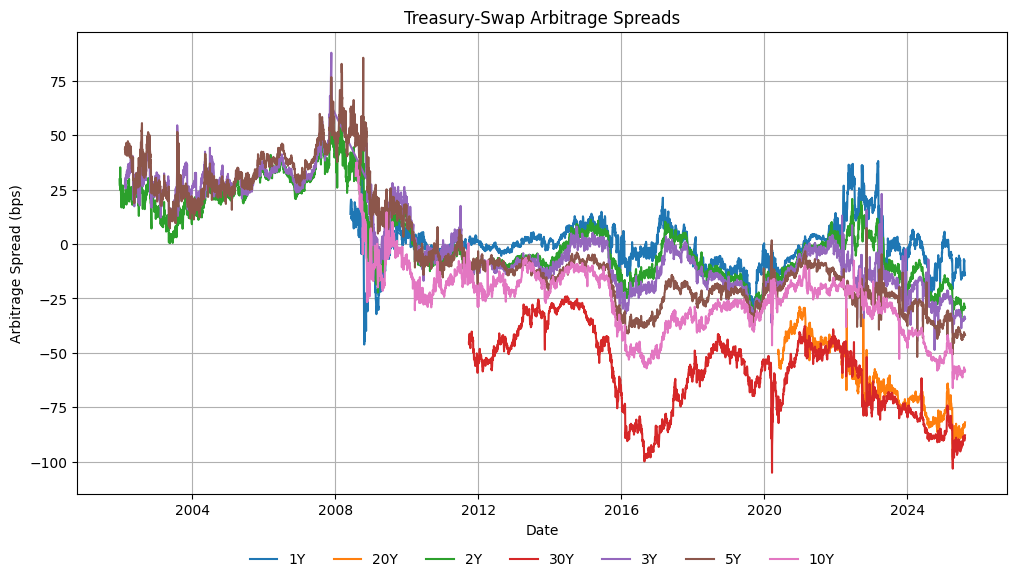
\includegraphics[width=0.8\textwidth]{\PathToAssets/treasury_swap_arbitrage_spreads.png}
  \vspace{0.2cm}

  \scriptsize
  Replicates persistently negative swap spreads documented in literature
\end{frame}

\begin{frame}
  \frametitle{Validation: GSCI Commodity Returns}
  \centering
  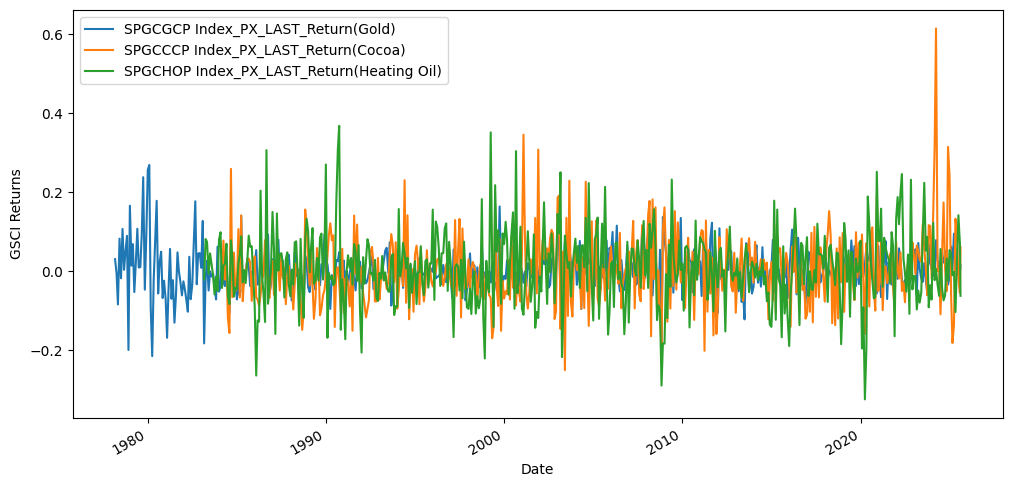
\includegraphics[width=0.8\textwidth]{\PathToAssets/commod_gsci_return.png}
  \vspace{0.2cm}

  \scriptsize
  24 GSCI commodity futures following canonical Yang (2013) methodology
\end{frame}

\begin{frame}
  \frametitle{Institutional Quality Data Sources}
  \begin{itemize}
  \item All datasets use institutional-grade data providers
  \item Industry-standard sources for financial research
  \item Strict adherence to canonical data cleaning procedures
  \item Next slide shows detailed data source mapping
  \end{itemize}
\end{frame}

\begin{frame}[plain]
  \tiny
  \vspace{-0.5cm}
  \centering
  \textbf{Data Sources by Dataset}\\
  \vspace{0.3cm}
  \begin{table}
  \centering
  \begin{tabular}{p{3cm}p{7cm}}
  \toprule
  Dataset Name & Data Sources \\
  \midrule
  CDS Contract & S\&P Global CDS (formerly Markit) \\
  Corporate Bond & WRDS TRACE, following Open Source Bond Asset Pricing \\
  CRSP Stock & Center for Research in Security Prices (CRSP) \\
  SPX Options & OptionMetrics IvyDB \\
  Treasury Bond & Center for Research in Security Prices \\
  CIP & Bloomberg Terminal \\
  Bank Cash Liquidity & WRDS Bank Regulatory Call Reports \\
  HKM Daily Factor & CRSP and Compustat, following He et al. (2017) \\
  Treasury Yield Curve & Board of Governors of the Federal Reserve System \\
  \bottomrule
  \end{tabular}
  \end{table}
\end{frame}

\begin{frame}
  \frametitle{Replication \& Validation Results}
  \label{slide:validation}
\begin{itemize}
\item \alert{Successfully replicated key results from canonical papers:}
\begin{itemize}
  \item Corporate bond credit spread patterns (Nozawa 2017)
  \item Options volatility risk premiums (Constantinides et al. 2013)
  \item CDS basis spread dynamics (Palhares 2012)
  \item Treasury yield curve characteristics (Gürkaynak et al. 2007)
\end{itemize}
\vspace{0.3cm}
\item \alert{Data quality validation:}
\begin{itemize}
  \item Cross-checked against published summary statistics
  \item Verified time series properties match literature
  \item Ensured no look-ahead bias in data construction
\end{itemize}
\vspace{0.3cm}
\item \alert{Open source code enables:}
\begin{itemize}
  \item Community validation and improvement
  \item Extension to new datasets and methods
  \item Elimination of researcher degrees of freedom
\end{itemize}
\end{itemize}
\end{frame}


%% Bibliographies are finicky in beamer.
%% References are cited inline manually throughout the presentation.
%% Full citations available in the working paper: github.com/jmbejara/ftsfr

\begin{frame}
  \frametitle{Repository \& Resources}
  \centering
  \vspace{1cm}
  \Large
  \alert{Paper \& Code:} \\
  \texttt{github.com/jmbejara/ftsfr}
  \vspace{1cm}

  \alert{Questions?}
  \vspace{0.5cm}

  \normalsize
  Contact: jeremiah.bejarano@ofr.treasury.gov
\end{frame}


\end{document}




